% architecture.tex -- the system as built: browser, dev proxy, FastAPI service, Assignment 2's runtime, files, optional parts
% COS30049 Assignment 3, Bitcoin Address Activity Explorer. Drawn from the code on main (13 Nov 2026).
% Compiles on its own:  pdflatex architecture.tex   (one cropped page; needs only tikz and lmodern).
% It does not use the standalone class, which a small TeX installation may lack; the last lines of
% this file crop the page to the picture instead. To place it in the report: 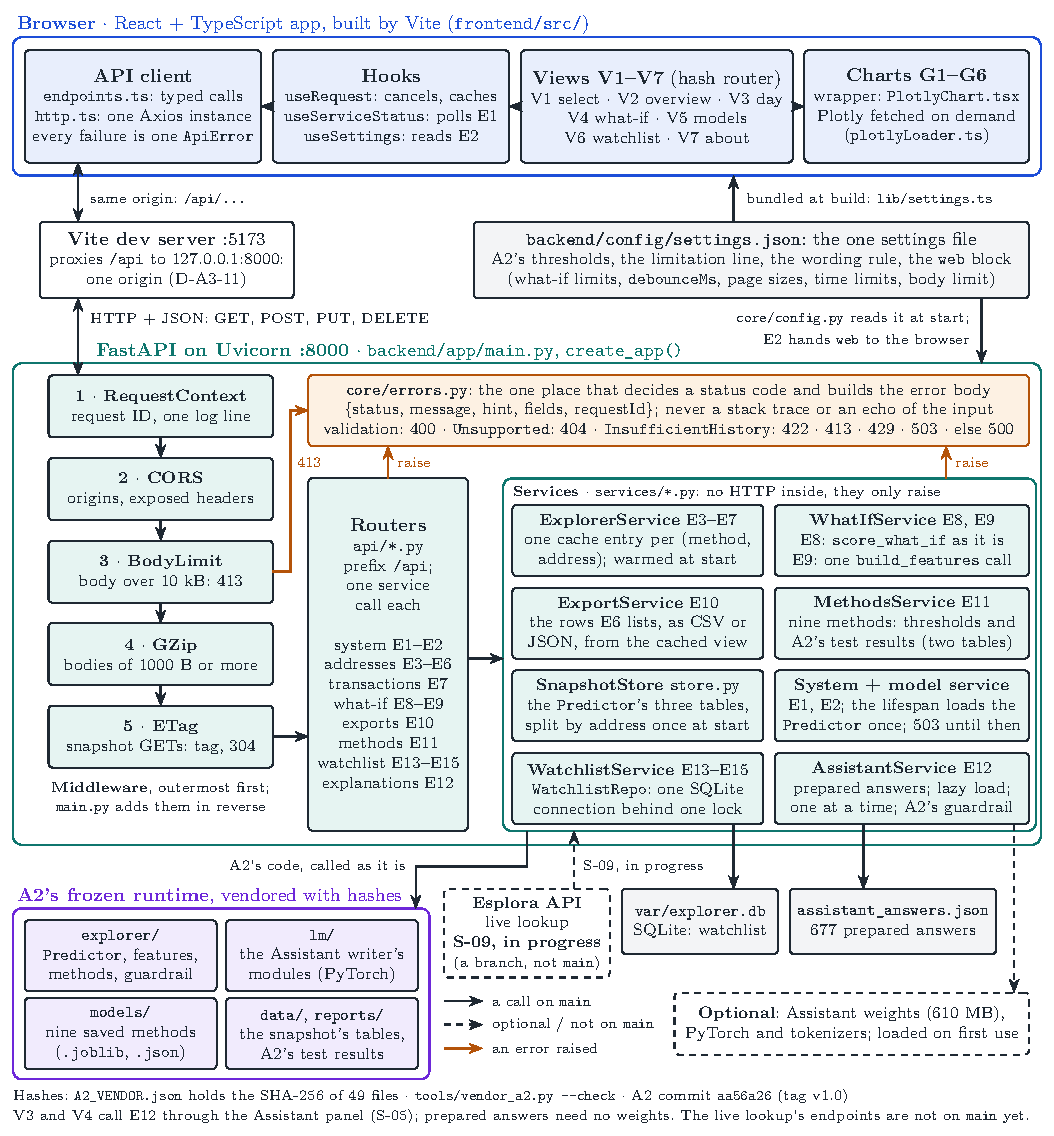
\includegraphics{architecture.pdf}.
% The boxes, words and arrows are the same as in architecture.svg; README.md lists the source file behind each.

\documentclass{article}
\usepackage[T1]{fontenc}
\usepackage{lmodern}
\usepackage{tikz}
\usetikzlibrary{arrows.meta, backgrounds}
% The plan's colours (docs/plan/main.tex).
\definecolor{ink}{HTML}{1F2933}
\definecolor{accent}{HTML}{1D4ED8}
\definecolor{accentsoft}{HTML}{E8EEFC}
\definecolor{teal}{HTML}{0F766E}
\definecolor{tealsoft}{HTML}{E6F4F2}
\definecolor{violet}{HTML}{6D28D9}
\definecolor{violetsoft}{HTML}{F1EBFD}
\definecolor{grey}{HTML}{6B7280}
\definecolor{greysoft}{HTML}{F3F4F6}
\definecolor{warn}{HTML}{B45309}
\definecolor{warnsoft}{HTML}{FDF1E3}
\pagestyle{empty}
\newsavebox{\figbox}
\newlength{\figborder}\setlength{\figborder}{6pt}
\begin{document}
\begin{lrbox}{\figbox}%
\frenchspacing
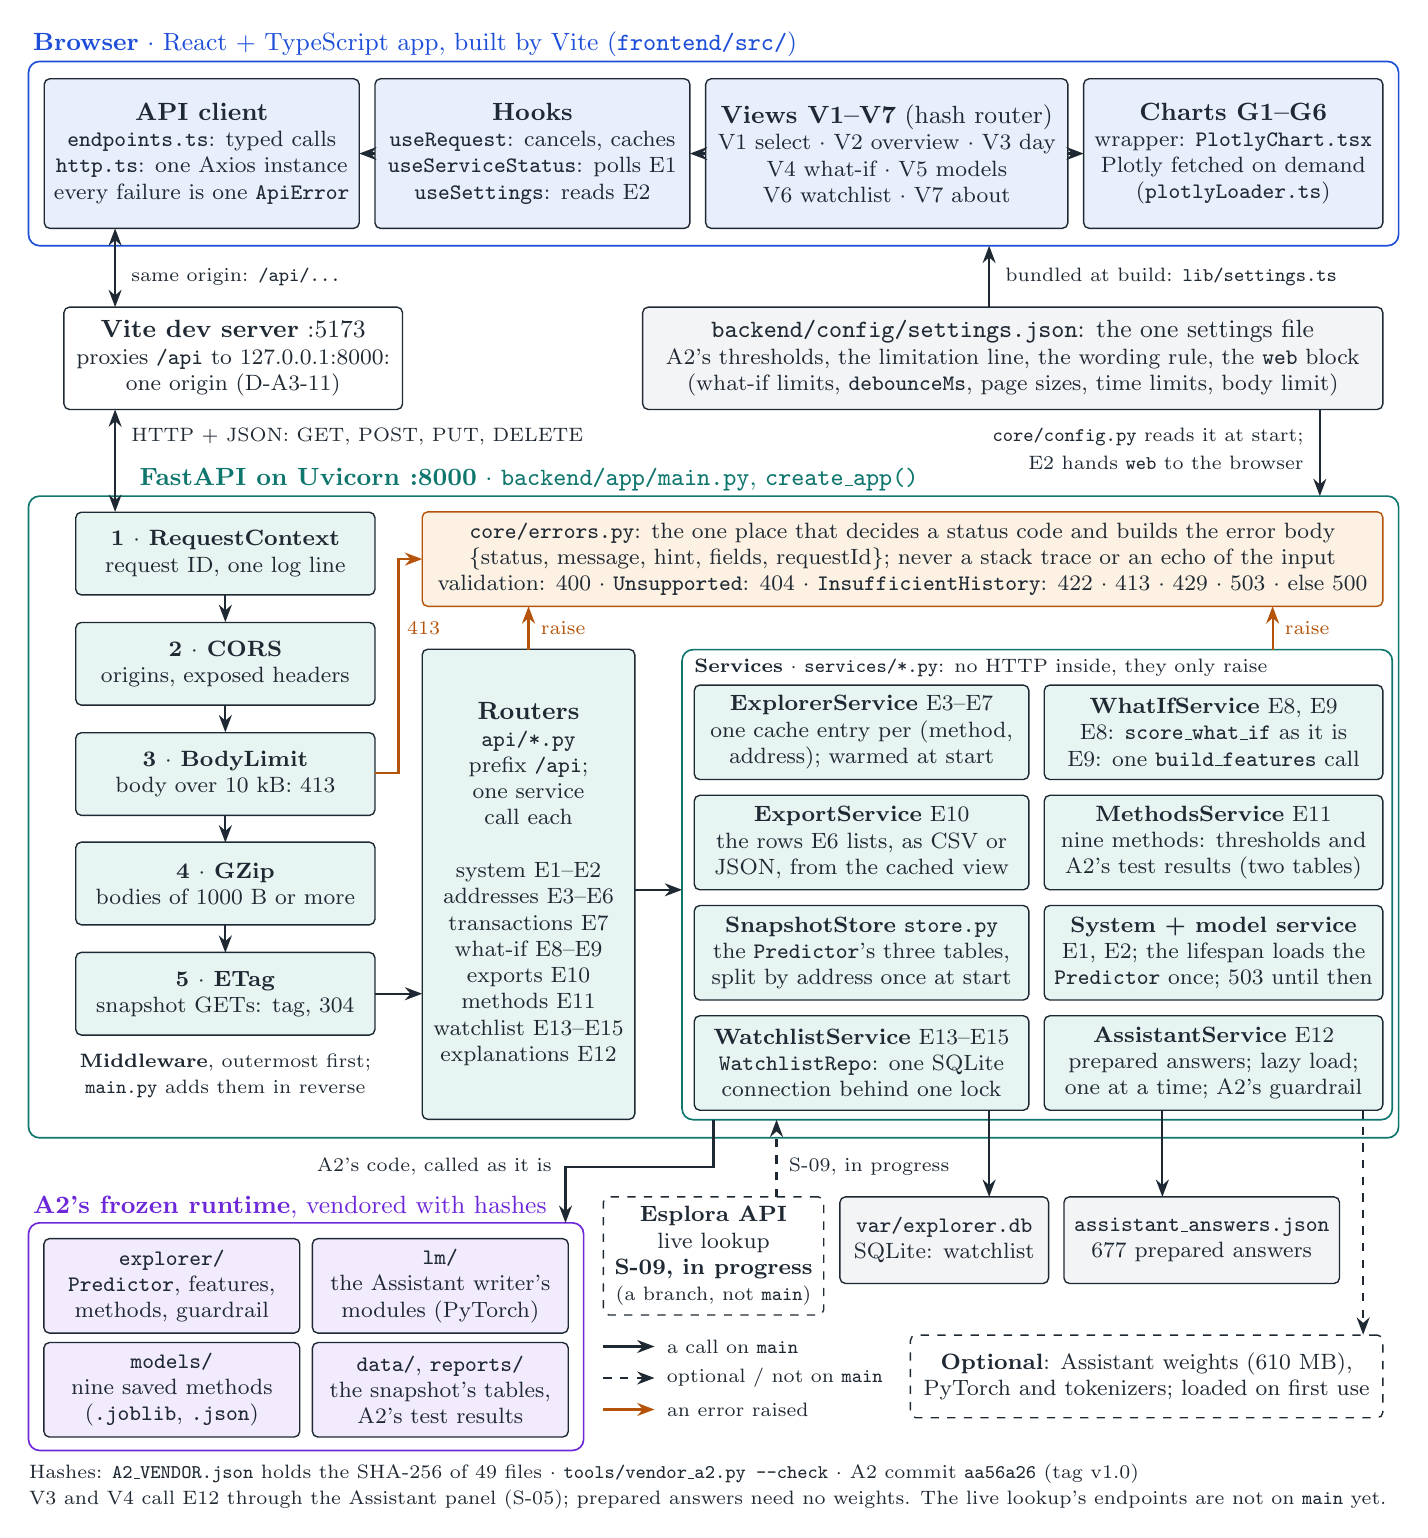
\begin{tikzpicture}[x=1cm, y=1cm, font=\footnotesize, text=ink,
  box/.style={draw=ink, rounded corners=2pt, align=center, inner sep=3pt, line width=0.5pt},
  fe/.style={box, fill=accentsoft}, be/.style={box, fill=tealsoft}, ml/.style={box, fill=violetsoft},
  st/.style={box, fill=greysoft}, er/.style={box, fill=warnsoft, draw=warn}, plain/.style={box, fill=white},
  txt/.style={align=center, inner sep=0pt},
  grp/.style={rounded corners=4pt, line width=0.6pt},
  arr/.style={-{Stealth[length=2.2mm]}, thick, draw=ink},
  darr/.style={{Stealth[length=2.2mm]}-{Stealth[length=2.2mm]}, thick, draw=ink},
  opt/.style={arr, dashed},
  err/.style={arr, draw=warn},
  bare/.style={thick, draw=ink}]
  % ---- groups (frames behind everything)
  \draw[grp, draw=accent] (-0.20,-2.12) rectangle (17.20,0.22);
  \node[anchor=south west, inner sep=1.5pt, text=accent, font=\small] at (-0.20,0.22) {\textbf{Browser} $\cdot$ React + TypeScript app, built by Vite (\texttt{frontend/src/})};
  \draw[grp, draw=teal] (-0.20,-13.45) rectangle (17.20,-5.30);
  \node[anchor=south west, inner sep=1.5pt, text=teal, font=\small] at (1.15,-5.30) {\textbf{FastAPI on Uvicorn :8000} $\cdot$ \texttt{backend/app/main.py}, \texttt{create\_app()}};
  \draw[grp, draw=teal] (8.10,-13.22) rectangle (17.12,-7.25);
  \draw[grp, draw=violet] (-0.20,-17.42) rectangle (6.85,-14.53);
  \node[anchor=south west, inner sep=1.5pt, text=violet, font=\small] at (-0.20,-14.53) {\textbf{A2's frozen runtime}, vendored with hashes};
  % ---- boxes
  \node[fe, minimum width=4.00cm, minimum height=1.90cm] (client) at (2.00,-0.95) {{\small \textbf{API client}}\\ \texttt{endpoints.ts}: typed calls\\ \texttt{http.ts}: one Axios instance\\ every failure is one \texttt{ApiError}};
  \node[fe, minimum width=4.00cm, minimum height=1.90cm] (hooks) at (6.20,-0.95) {{\small \textbf{Hooks}}\\ \texttt{useRequest}: cancels, caches\\ \texttt{useServiceStatus}: polls E1\\ \texttt{useSettings}: reads E2};
  \node[fe, minimum width=4.60cm, minimum height=1.90cm] (views) at (10.70,-0.95) {{\small \textbf{Views V1--V7} (hash router)}\\ V1 select $\cdot$ V2 overview $\cdot$ V3 day\\ V4 what-if $\cdot$ V5 models\\ V6 watchlist $\cdot$ V7 about};
  \node[fe, minimum width=3.80cm, minimum height=1.90cm] (charts) at (15.10,-0.95) {{\small \textbf{Charts G1--G6}}\\ wrapper: \texttt{PlotlyChart.tsx}\\ Plotly fetched on demand\\ (\texttt{plotlyLoader.ts})};
  \node[plain, minimum width=4.30cm, minimum height=1.30cm] (proxy) at (2.40,-3.55) {{\small \textbf{Vite dev server} :5173}\\ proxies \texttt{/api} to 127.0.0.1:8000:\\ one origin (D-A3-11)};
  \node[st, minimum width=9.40cm, minimum height=1.30cm] (settings) at (12.30,-3.55) {{\small \textbf{\texttt{backend/config/settings.json}}: the one settings file}\\ A2's thresholds, the limitation line, the wording rule, the \texttt{web} block\\ (what-if limits, \texttt{debounceMs}, page sizes, time limits, body limit)};
  \node[be, minimum width=3.80cm, minimum height=1.05cm] (mw1) at (2.30,-6.03) {\textbf{1 $\cdot$ RequestContext}\\ request ID, one log line};
  \node[be, minimum width=3.80cm, minimum height=1.05cm] (mw2) at (2.30,-7.43) {\textbf{2 $\cdot$ CORS}\\ origins, exposed headers};
  \node[be, minimum width=3.80cm, minimum height=1.05cm] (mw3) at (2.30,-8.83) {\textbf{3 $\cdot$ BodyLimit}\\ body over 10 kB: 413};
  \node[be, minimum width=3.80cm, minimum height=1.05cm] (mw4) at (2.30,-10.22) {\textbf{4 $\cdot$ GZip}\\ bodies of 1000 B or more};
  \node[be, minimum width=3.80cm, minimum height=1.05cm] (mw5) at (2.30,-11.62) {\textbf{5 $\cdot$ ETag}\\ snapshot GETs: tag, 304};
  \node[er, minimum width=12.20cm, minimum height=1.20cm] (errors) at (10.90,-6.10) {\textbf{\texttt{core/errors.py}}: the one place that decides a status code and builds the error body\\ \{status, message, hint, fields, requestId\}; never a stack trace or an echo of the input\\ validation: 400 $\cdot$ \texttt{Unsupported}: 404 $\cdot$ \texttt{InsufficientHistory}: 422 $\cdot$ 413 $\cdot$ 429 $\cdot$ 503 $\cdot$ else 500};
  \node[be, minimum width=2.70cm, minimum height=5.97cm] (routers) at (6.15,-10.23) {{\small \textbf{Routers}}\\ \texttt{api/*.py}\\ prefix \texttt{/api};\\ one service\\ call each\\ \\ system  E1--E2\\ addresses  E3--E6\\ transactions  E7\\ what-if  E8--E9\\ exports  E10\\ methods  E11\\ watchlist  E13--E15\\ explanations  E12};
  \node[be, minimum width=4.25cm, minimum height=1.20cm] (s_explorer) at (10.38,-8.30) {\textbf{ExplorerService} E3--E7\\ one cache entry per (method,\\ address); warmed at start};
  \node[be, minimum width=4.30cm, minimum height=1.20cm] (s_whatif) at (14.85,-8.30) {\textbf{WhatIfService} E8, E9\\ E8: \texttt{score\_what\_if} as it is\\ E9: one \texttt{build\_features} call};
  \node[be, minimum width=4.25cm, minimum height=1.20cm] (s_export) at (10.38,-9.70) {\textbf{ExportService} E10\\ the rows E6 lists, as CSV or\\ JSON, from the cached view};
  \node[be, minimum width=4.30cm, minimum height=1.20cm] (s_methods) at (14.85,-9.70) {\textbf{MethodsService} E11\\ nine methods: thresholds and\\ A2's test results (two tables)};
  \node[be, minimum width=4.25cm, minimum height=1.20cm] (s_store) at (10.38,-11.10) {\textbf{SnapshotStore} \texttt{store.py}\\ the \texttt{Predictor}'s three tables,\\ split by address once at start};
  \node[be, minimum width=4.30cm, minimum height=1.20cm] (s_system) at (14.85,-11.10) {\textbf{System + model service}\\ E1, E2; the lifespan loads the\\ \texttt{Predictor} once; 503 until then};
  \node[be, minimum width=4.25cm, minimum height=1.20cm] (s_watch) at (10.38,-12.50) {\textbf{WatchlistService} E13--E15\\ \texttt{WatchlistRepo}: one SQLite\\ connection behind one lock};
  \node[be, minimum width=4.30cm, minimum height=1.20cm] (s_assist) at (14.85,-12.50) {\textbf{AssistantService} E12\\ prepared answers; lazy load;\\ one at a time; A2's guardrail};
  \node[ml, minimum width=3.25cm, minimum height=1.20cm] (a_explorer) at (1.62,-15.33) {\textbf{\texttt{explorer/}}\\ \texttt{Predictor}, features,\\ methods, guardrail};
  \node[ml, minimum width=3.25cm, minimum height=1.20cm] (a_lm) at (5.03,-15.33) {\textbf{\texttt{lm/}}\\ the Assistant writer's\\ modules (PyTorch)};
  \node[ml, minimum width=3.25cm, minimum height=1.20cm] (a_models) at (1.62,-16.65) {\textbf{\texttt{models/}}\\ nine saved methods\\ (\texttt{.joblib}, \texttt{.json})};
  \node[ml, minimum width=3.25cm, minimum height=1.20cm] (a_data) at (5.03,-16.65) {\textbf{\texttt{data/}}, \textbf{\texttt{reports/}}\\ the snapshot's tables,\\ A2's test results};
  \node[plain, dashed, minimum width=2.80cm, minimum height=1.50cm] (esplora) at (8.50,-14.95) {\textbf{Esplora API}\\ live lookup\\ \textbf{S-09, in progress}\\ {\scriptsize (a branch, not \texttt{main})}};
  \node[st, minimum width=2.65cm, minimum height=1.10cm] (db) at (11.43,-14.75) {\textbf{\texttt{var/explorer.db}}\\ SQLite: watchlist};
  \node[st, minimum width=3.50cm, minimum height=1.10cm] (answers) at (14.70,-14.75) {\textbf{\texttt{assistant\_answers.json}}\\ 677 prepared answers};
  \node[plain, dashed, minimum width=6.00cm, minimum height=1.05cm] (weights) at (14.00,-16.48) {\textbf{Optional}: Assistant weights (610 MB),\\ PyTorch and tokenizers; loaded on first use};
  % ---- arrows
  % views -> hooks
  \draw[arr] (8.40,-0.95) -- (8.20,-0.95);
  % hooks -> client
  \draw[arr] (4.20,-0.95) -- (4.00,-0.95);
  % views -> charts
  \draw[arr] (13.00,-0.95) -- (13.20,-0.95);
  % client <-> proxy
  \draw[darr] (0.90,-1.90) -- (0.90,-2.90);
  % proxy <-> RequestContext (outermost middleware)
  \draw[darr] (0.90,-4.20) -- (0.90,-5.50);
  % settings.json -> browser (bundled)
  \draw[arr] (12.00,-2.90) -- (12.00,-2.12);
  % settings.json -> FastAPI (core/config.py)
  \draw[arr] (16.20,-4.20) -- (16.20,-5.30);
  % middleware 1 -> 2
  \draw[arr] (2.30,-6.55) -- (2.30,-6.90);
  % middleware 2 -> 3
  \draw[arr] (2.30,-7.95) -- (2.30,-8.30);
  % middleware 3 -> 4
  \draw[arr] (2.30,-9.35) -- (2.30,-9.70);
  % middleware 4 -> 5
  \draw[arr] (2.30,-10.75) -- (2.30,-11.10);
  % ETag (innermost) -> routers
  \draw[arr] (4.20,-11.62) -- (4.80,-11.62);
  % routers -> services
  \draw[arr] (7.50,-10.30) -- (8.10,-10.30);
  % BodyLimit -> core/errors.py (413, handle_api_error)
  \draw[err] (4.20,-8.82) -- (4.50,-8.82) -- (4.50,-6.10) -- (4.80,-6.10);
  % routers raise -> core/errors.py
  \draw[err] (6.15,-7.25) -- (6.15,-6.70);
  % services raise -> core/errors.py
  \draw[err] (15.60,-7.25) -- (15.60,-6.70);
  % services -> A2 runtime
  \draw[arr] (8.50,-13.22) -- (8.50,-13.82) -- (6.62,-13.82) -- (6.62,-14.53);
  % live lookup -> services (S-09, in progress; not on main)
  \draw[opt] (9.30,-14.20) -- (9.30,-13.22);
  % WatchlistRepo -> SQLite file
  \draw[arr] (12.00,-13.10) -- (12.00,-14.20);
  % AssistantService -> prepared answers
  \draw[arr] (14.20,-13.10) -- (14.20,-14.20);
  % AssistantService -> weights and torch (optional)
  \draw[opt] (16.75,-13.10) -- (16.75,-15.95);
  \draw[arr] (7.10,-16.10) -- (7.75,-16.10);
  \draw[opt] (7.10,-16.50) -- (7.75,-16.50);
  \draw[err] (7.10,-16.90) -- (7.75,-16.90);
  % ---- labels
  \node[txt, anchor=west, font=\scriptsize] at (1.10,-2.52) {same origin: \texttt{/api/...}};
  \node[txt, anchor=west, font=\scriptsize] at (1.10,-4.55) {HTTP + JSON: GET, POST, PUT, DELETE};
  \node[txt, anchor=west, font=\scriptsize] at (12.20,-2.52) {bundled at build: \texttt{lib/settings.ts}};
  \node[txt, anchor=east, font=\scriptsize] at (16.00,-4.55) {\texttt{core/config.py} reads it at start;};
  \node[txt, anchor=east, font=\scriptsize] at (16.00,-4.88) {E2 hands \texttt{web} to the browser};
  \node[txt, font=\scriptsize] at (2.30,-12.50) {\textbf{Middleware}, outermost first;};
  \node[txt, font=\scriptsize] at (2.30,-12.83) {\texttt{main.py} adds them in reverse};
  \node[txt, anchor=west, font=\scriptsize] at (8.25,-7.48) {\textbf{Services} $\cdot$ \texttt{services/*.py}: no HTTP inside, they only raise};
  \node[txt, anchor=west, text=warn, font=\scriptsize] at (4.60,-6.98) {413};
  \node[txt, anchor=west, text=warn, font=\scriptsize] at (6.30,-6.98) {raise};
  \node[txt, anchor=west, text=warn, font=\scriptsize] at (15.75,-6.98) {raise};
  \node[txt, anchor=east, font=\scriptsize] at (6.45,-13.82) {A2's code, called as it is};
  \node[txt, anchor=west, font=\scriptsize] at (-0.20,-17.72) {Hashes: \texttt{A2\_VENDOR.json} holds the SHA-256 of 49 files $\cdot$ \texttt{tools/vendor\_a2.py -{}-{}check} $\cdot$ A2 commit \texttt{aa56a26} (tag v1.0)};
  \node[txt, anchor=west, font=\scriptsize] at (-0.20,-18.05) {V3 and V4 call E12 through the Assistant panel (S-05); prepared answers need no weights. The live lookup's endpoints are not on \texttt{main} yet.};
  \node[txt, anchor=west, font=\scriptsize] at (9.45,-13.82) {S-09, in progress};
  \node[txt, anchor=west, font=\scriptsize] at (7.90,-16.10) {a call on \texttt{main}};
  \node[txt, anchor=west, font=\scriptsize] at (7.90,-16.50) {optional / not on \texttt{main}};
  \node[txt, anchor=west, font=\scriptsize] at (7.90,-16.90) {an error raised};
\end{tikzpicture}%
\end{lrbox}
% One page, cropped to the picture plus a 6 pt border (what the standalone class would do).
\pdfpagewidth=\dimexpr\wd\figbox+2\figborder\relax
\pdfpageheight=\dimexpr\ht\figbox+\dp\figbox+2\figborder\relax
\pdfhorigin=\figborder \pdfvorigin=\figborder
\hoffset=0pt \voffset=0pt
\shipout\vbox{\box\figbox}
\end{document}
